\subsection{Diseño de Objetos de Clasificación}

Los objetos de clasificación constituyen los elementos manipulables del kit que los estudiantes programarán al robot para detectar, recoger y depositar en las zonas correspondientes. Su diseño debe equilibrar facilidad de detección por visión por computador, compatibilidad con el sistema de succión por vacío y robustez operativa.

\subsubsection{Requerimientos de Diseño}

Los objetos de clasificación deben cumplir los siguientes criterios:

\paragraph{Requerimientos Geométricos}

\begin{itemize}
    \item Dimensión característica base: 25 mm × 25 mm (compatible con ventosa Ø15 mm con holgura de 5 mm)
    \item Altura uniforme: 25 mm para todos los objetos
    \item Geometrías distinguibles mediante algoritmos de detección de formas
    \item Superficie superior plana y lisa para contacto óptimo con ventosa
    \item Estabilidad cuando se colocan sobre superficie plana
\end{itemize}

\paragraph{Requerimientos de Percepción Visual}

\begin{itemize}
    \item Color uniforme y distinguible del entorno
    \item Contraste elevado respecto a fondo blanco (zona de recolección) y negro (plataforma base)
    \item Diferenciación respecto a colores de zonas de depósito (rojo, verde, azul, amarillo)
    \item Superficie mate para minimizar reflejos bajo iluminación artificial
\end{itemize}

\subsubsection{Geometrías Seleccionadas}

Se diseñaron cuatro geometrías básicas distinguibles tanto por forma como por número de vértices o curvatura. La Figura \ref{fig:objetosRecoleccion} presenta las dimensiones de cada tipo.

\begin{figure}[H]
    \centering
    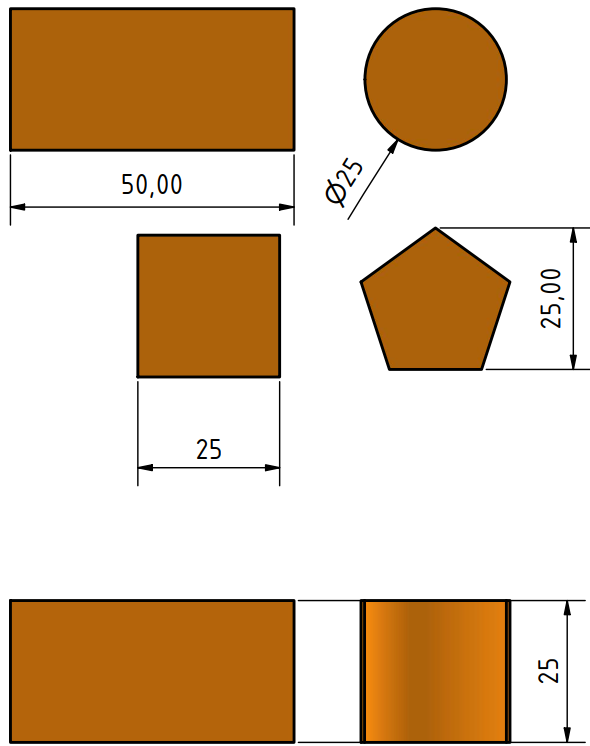
\includegraphics[width=0.4\textwidth]{06disenoConceptual/img/zonaRecoleccion/objetosRecoleccion.png}
    \caption{Geometrías de objetos de clasificación con dimensiones principales. Superior izquierda: Rectángulo 50 mm × 25 mm. Superior centro: Cuadrado 25 mm × 25 mm. Superior derecha: Círculo Ø25 mm. Centro derecha: Pentágono regular inscrito en círculo de 25 mm de diámetro. Inferior: Vista lateral mostrando altura uniforme de 25 mm para todos los objetos. Color: Naranja uniforme.}
    \label{fig:objetosRecoleccion}
\end{figure}

\paragraph{Cuadrado (25 mm × 25 mm)}

\begin{itemize}
    \item Dimensiones: 25 mm × 25 mm × 25 mm (cubo perfecto)
    \item Características: 4 vértices, 4 lados iguales, relación aspecto 1:1
    \item Ventaja didáctica: Forma más simple, facilita validación inicial de algoritmos
\end{itemize}

\paragraph{Rectángulo (50 mm × 25 mm)}

\begin{itemize}
    \item Dimensiones: 50 mm × 25 mm × 25 mm
    \item Características: 4 vértices, relación aspecto 2:1
    \item Ventaja didáctica: Introduce concepto de orientación (eje mayor/menor)
\end{itemize}

\paragraph{Círculo (Ø25 mm)}

\begin{itemize}
    \item Dimensiones: Ø25 mm × 25 mm de altura
    \item Características: Ausencia de vértices, geometría circular perfecta
    \item Ventaja didáctica: Invarianza a rotación, prueba de algoritmos de circularidad
\end{itemize}

\paragraph{Pentágono Regular (Ø25 mm circunscrito)}

\begin{itemize}
    \item Dimensiones: Pentágono regular inscrito en círculo Ø25 mm, altura 25 mm
    \item Características: 5 vértices, ángulos internos de 108°
    \item Ventaja didáctica: Forma más compleja, requiere algoritmos robustos de detección de vértices
\end{itemize}

\subsubsection{Selección de Color}

Se seleccionó el color naranja como color uniforme para todos los objetos de clasificación, fundamentado en criterios de diferenciación cromática.

\paragraph{Contraste con Elementos del Sistema}

El naranja proporciona máxima diferenciación respecto a todos los elementos cromáticos del kit:

\begin{itemize}
    \item \textbf{Plataforma base}: Negro, contraste por luminosidad muy elevado
    \item \textbf{Zona de recolección}: Blanca, contraste por saturación
    \item \textbf{Zonas de depósito}: Rojo, verde, azul y amarillo, diferenciable por tonalidad
\end{itemize}

Esta diferenciación cromática facilita la segmentación de objetos mediante algoritmos de procesamiento de imágenes, permitiendo detección robusta bajo condiciones de iluminación artificial típicas de laboratorio.

\subsubsection{Material de Fabricación}

Los objetos se fabrican mediante FDM utilizando TPU (poliuretano termoplástico) en color naranja. La selección de TPU se fundamenta en su flexibilidad, que proporciona ventajas significativas:

\begin{itemize}
    \item \textbf{Mayor adherencia a la ventosa}: La superficie flexible del TPU se adapta mejor a la geometría de la ventosa de silicona, mejorando el sellado y la fuerza de succión
    \item \textbf{Resistencia a impactos}: El material flexible absorbe energía durante manipulación, reduciendo riesgo de fractura por caídas o colisiones
    \item \textbf{Amortiguación}: La flexibilidad reduce el impacto que el  objeto tiene en la pinza del robot.
\end{itemize}
